\documentclass{eusflat2021}

\title{\bf Ifsa-Eusflat 2021 Bratislava: Instructions for Authors}
\author{Author$^a$ \and $^*$Corresponding Author$^b$ \and Author$^{b,c}$\\
$^a$Department, Faculty, University, Address, \email{account@domain.com} \\
$^b$Department, Faculty, University, Address, \email{account@domain.com} \\
$^c$Department, Faculty, University, Address, \email{account@domain.com}}

\begin{document}

\maketitle

\begin{abstract}
The abstract must be indented 0.7 cm both on left as well as right-hand margins.

Please, do not place or cite tables and figures in the abstract.

{\bf Keywords:} Start with capital, Use comma, At least three keywords.
\end{abstract}

\section{General formatting instructions}

\begin{enumerate}
    \item Please, do not modify the two-column layout of the page and leave margins as they are: 3.17~cm on top and bottom and 2.50~cm for the left and right margins except for the first page, which has different margin at the top: 4.44~cm.
    
    \item Please, do not modify the font of the normal text. The normal text should be in Times New Roman 10 points.

    \item Please don’t add any information in headers or footers such as page numbers.

    \item Please make sure the article contains all necessary elements of a scientific paper (title, abstract, keywords, introduction, conclusion, etc.) Atlantis Press, furthermore, strongly advises adding an “Authors Contribution” and an “Acknowledgement” section at the end of the article, before the references.

    \item {\bf Article title must NOT be written in upper case letters.} Italics, sub- and superscript are the only formatting elements that are accepted in article titles. Math symbols and non-Latin characters can be used too.
    
    \item Please mark the corresponding author with an asterisk $^*$ (If no author is marked with an asterisk, per default, we will consider the first author as the corresponding author.)

    \item Figures and tables should be placed either at the top or bottom of the page and close to the text referring to them if possible. They shouldn’t span over several columns except in the case of very large tables.

    \item Section title should always be followed by text, i.e. not be at the very end of a column or a page.
\end{enumerate}

Submitted full papers are to be supposed to be of at least 4 pages length. The authors should submit their papers electronically, written in English, due to the given deadline, through a web upload procedure available, see \mbox{\url{http://ifsa-eusflat2021.eu}}.

The only allowed format for the submission is PDF.

MS Word and LaTeX{} style and template files are available in the Conference web page.

\section{Footnotes and Citations}

Footnotes must be numbered\footnote{Example of footnote.}, and placed at the bottom of the column where they appear.

Citations must include the reference number between brackets, for example, one citation \cite{Zadeh75} or two citations \cite{Zadeh75b,Zadeh75c}. All three cited references are articles, see below. In order to see the format of different types, e.g. books \cite{Gottwald93,NovakPerfilievaMockor99,KlementMesiarPap00}, articles in collections (edited books) \cite{BandlerKohout80b,NavaraPetrik_EUSFLAT07}, articles in conference proceedings \cite{DuboisNakata_IFSA97}, or Ph.D. thesis \cite{EsterPhD}, see the references below. References must be sorted by the author's name. Use the attached BST style file \url{eusflat2021.bst} for the correct appearance of your references.

\section{Tables}

All tables must be centered and clear (See Table \ref{table}).
\begin{table}[ht]
\begin{center}
\vspace{1ex}
\begin{tabular}{|c|c|} \hline
    {\bf NAME} & {\bf AGE} \\\hline
    John Smith &   35\\
    George Brown & 21 \\ \hline
\end{tabular}
\caption{\label{table}The number and caption of the table always appear below the table.}
\end{center}
\end{table}

\section{Figures}

All figures must be centered like Figure~\ref{figure1}.
\begin{figure}[ht]
\begin{center}
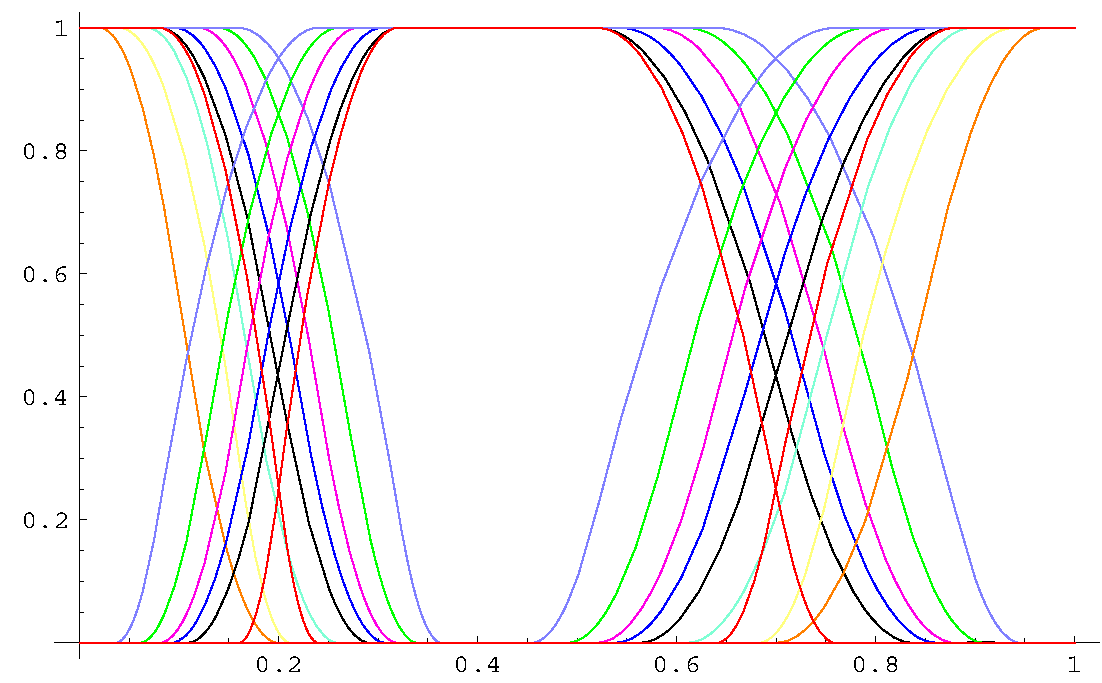
\includegraphics[width=0.9\columnwidth]{FuzzySets}
  \caption{\label{figure1}The number and caption
of the figure must always appear below the figure.}
\end{center}
\end{figure}

\begin{acknowledgment}
    For the acknowledgement use predefined environment. The word ``Acknowledgement'' must be aligned to the left, boldfaced and not numbered.
\end{acknowledgment}

\bibliographystyle{eusflat2021}
\bibliography{BIBeusflat2021}

%\begin{thebibliography}{99}
%
% For manual entries if no bib file database is used
%
% In such case, be careful in meeting the same format.
%
%\end{thebibliography}

\end{document}
